% This is "sig-alternate.tex" V1.9 April 2009
% This file should be compiled with V2.4 of "sig-alternate.cls" April 2009
%
% This example file demonstrates the use of the 'sig-alternate.cls'
% V2.4 LaTeX2e document class file. It is for those submitting
% articles to ACM Conference Proceedings WHO DO NOT WISH TO
% STRICTLY ADHERE TO THE SIGS (PUBS-BOARD-ENDORSED) STYLE.
% The 'sig-alternate.cls' file will produce a similar-looking,
% albeit, 'tighter' paper resulting in, invariably, fewer pages.
%
% ----------------------------------------------------------------------------------------------------------------
% This .tex file (and associated .cls V2.4) produces:
%       1) The Permission Statement
%       2) The Conference (location) Info information
%       3) The Copyright Line with ACM data
%       4) NO page numbers
%
% as against the acm_proc_article-sp.cls file which
% DOES NOT produce 1) thru' 3) above.
%
% Using 'sig-alternate.cls' you have control, however, from within
% the source .tex file, over both the CopyrightYear
% (defaulted to 200X) and the ACM Copyright Data
% (defaulted to X-XXXXX-XX-X/XX/XX).
% e.g.
% \CopyrightYear{2007} will cause 2007 to appear in the copyright line.
% \crdata{0-12345-67-8/90/12} will cause 0-12345-67-8/90/12 to appear in the copyright line.
%
% ---------------------------------------------------------------------------------------------------------------
% This .tex source is an example which *does* use
% the .bib file (from which the .bbl file % is produced).
% REMEMBER HOWEVER: After having produced the .bbl file,
% and prior to final submission, you *NEED* to 'insert'
% your .bbl file into your source .tex file so as to provide
% ONE 'self-contained' source file.
%
% ================= IF YOU HAVE QUESTIONS =======================
% Questions regarding the SIGS styles, SIGS policies and
% procedures, Conferences etc. should be sent to
% Adrienne Griscti (griscti@acm.org)
%
% Technical questions _only_ to
% Gerald Murray (murray@hq.acm.org)
% ===============================================================
%
% For tracking purposes - this is V1.9 - April 2009

\documentclass{sig-alternate}
\usepackage{algorithm}
\usepackage{algorithmic}
\usepackage{url}
\begin{document}
%
% --- Author Metadata here ---
\conferenceinfo{ICCAD}{'11 San Jose, CA USA}
\CopyrightYear{2011} % Allows default copyright year (200X) to be over-ridden - IF NEED BE.
\crdata{978-1-60558-800-1/09/11}  % Allows default copyright data (0-89791-88-6/97/05) to be over-ridden - IF NEED BE.
% --- End of Author Metadata ---

\title{Inferring Assertion for Complementary Synthesis}
%\subtitle{[Extended Abstract]
%\titlenote{A full version of this paper is available as
%\textit{Author's Guide to Preparing ACM SIG Proceedings Using
%\LaTeX$2_\epsilon$\ and BibTeX} at
%\texttt{www.acm.org/eaddress.htm}}}
%
% You need the command \numberofauthors to handle the 'placement
% and alignment' of the authors beneath the title.
%
% For aesthetic reasons, we recommend 'three authors at a time'
% i.e. three 'name/affiliation blocks' be placed beneath the title.
%
% NOTE: You are NOT restricted in how many 'rows' of
% "name/affiliations" may appear. We just ask that you restrict
% the number of 'columns' to three.
%
% Because of the available 'opening page real-estate'
% we ask you to refrain from putting more than six authors
% (two rows with three columns) beneath the article title.
% More than six makes the first-page appear very cluttered indeed.
%
% Use the \alignauthor commands to handle the names
% and affiliations for an 'aesthetic maximum' of six authors.
% Add names, affiliations, addresses for
% the seventh etc. author(s) as the argument for the
% \additionalauthors command.
% These 'additional authors' will be output/set for you
% without further effort on your part as the last section in
% the body of your article BEFORE References or any Appendices.

\numberofauthors{4} %  in this sample file, there are a *total*
% of EIGHT authors. SIX appear on the 'first-page' (for formatting
% reasons) and the remaining two appear in the \additionalauthors section.
%
\author{
%% You can go ahead and credit any number of authors here,
%% e.g. one 'row of three' or two rows (consisting of one row of three
%% and a second row of one, two or three).
%%
%% The command \alignauthor (no curly braces needed) should
%% precede each author name, affiliation/snail-mail address and
%% e-mail address. Additionally, tag each line of
%% affiliation/address with \affaddr, and tag the
%% e-mail address with \email.
%%
%% 1st. author
\alignauthor
%%Ben Trovato\titlenote{Dr.~Trovato insisted his name be first.}\\
ShengYu Shen\\
       \affaddr{School of Computer Science, National University of Defense Technology}\\
       \affaddr{410073,DeYa Avenue}\\
       \affaddr{ChangSha,China}\\
       \email{syshen@nudt.edu.cn}
% 2nd. author
\alignauthor
%G.K.M. Tobin\titlenote{The secretary disavows any knowledge of this author's actions.}\\
JianMin Zhang\\
       \affaddr{School of Computer Science, National University of Defense Technology}\\
       \affaddr{410073,DeYa Avenue}\\
       \affaddr{ChangSha,China}\\
       \email{jmzhang@nudt.edu.cn}
% 3rd. author
%\alignauthor Lars Th{\o}rv{\"a}ld\titlenote{This author is the one who did all the really hard work.}\\
\alignauthor
Ying Qin\\
       \affaddr{School of Computer Science, National University of Defense Technology}\\
       \affaddr{410073,DeYa Avenue}\\
       \affaddr{ChangSha,China}\\
       \email{qy123@nudt.edu.cn}
\and  % use '\and' if you need 'another row' of author names
% 4th. author
\alignauthor
%Lawrence P. Leipuner\\
SiKun Li\\
       \affaddr{School of Computer Science, National University of Defense Technology}\\
       \affaddr{410073,DeYa Avenue}\\
       \affaddr{ChangSha,China}\\
       \email{skli@nudt.edu.cn}
%% 5th. author
%%\alignauthor Sean Fogarty\\
%%       \affaddr{NASA Ames Research Center}\\
%%       \affaddr{Moffett Field}\\
%%       \affaddr{California 94035}\\
%%       \email{fogartys@amesres.org}
%% 6th. author
%%\alignauthor Charles Palmer\\
%%       \affaddr{Palmer Research Laboratories}\\
%%       \affaddr{8600 Datapoint Drive}\\
%%       \affaddr{San Antonio, Texas 78229}\\
%%       \email{cpalmer@prl.com}
}
% There's nothing stopping you putting the seventh, eighth, etc.
% author on the opening page (as the 'third row') but we ask,
% for aesthetic reasons that you place these 'additional authors'
% in the \additional authors block, viz.
%\additionalauthors{Additional authors: John Smith (The Th{\o}rv{\"a}ld Group,
%email: {\texttt{jsmith@affiliation.org}}) and Julius P.~Kumquat
%(The Kumquat Consortium, email: {\texttt{jpkumquat@consortium.net}}).}
%\date{30 July 1999}
% Just remember to make sure that the TOTAL number of authors
% is the number that will appear on the first page PLUS the
% number that will appear in the \additionalauthors section.

\maketitle
\begin{abstract}
Complementary synthesis can automatically synthesize the decoder circuit of an encoder.
However,
its user needs to manually specify an assertion on some configuration pins
to prevent the encoder from reaching the non-working states.
To avoid this tedious job,
we propose an automatic approach to infer this assertion.

\textbf{First},
we propose a halting algorithm that can decide the existence of the decoder for every particular assertion.
\textbf{Second},
for every invalid value of configuration pins that leads to the non-existence of the decoder,
we use cofactoring and Craig interpolation to infer a new formula,
which covers a larger set of such invalid values.
This second step is repeated until all invalid values are covered by these inferred formulas.
\textbf{Finally},
we obtain the final assertion by anding the inverses of all these inferred formulas.
The decoder exists if and only if this final assertion is still satisfiable.

To illustrate its usefulness,
we have run our algorithm on several complex encoder circuits,
including PCI-E and Ethernet.
Experimental results show that
our algorithm can always infer assertions for them.
\end{abstract}

% A category with the (minimum) three required fields
%\category{H.4}{Information Systems Applications}{Miscellaneous}
%A category including the fourth, optional field follows...
%\category{D.2.8}{Software Engineering}{Metrics}[complexity measures, performance measures]
\category{B.5.2}{REGISTER-TRANSFER-LEVEL IMPLEMENTATION}{Design Aids}[Automatic synthesis]
\category{B.4.4}{ INPUT/OUTPUT AND DATA COMMUNICATIONS}{Performance Analysis and Design Aids}[Formal models]

\terms{Algorithms, Design, Theory, Verification}

\keywords{Complementary Synthesis, Inferring Assertion, Cofactoring, Craig Interpolation} % NOT required for Proceedings
\newtheorem{algo}{Algorithm}
\newtheorem{lemma}{\textbf{Lemma}}
\newtheorem{theorem}{\textbf{Theorem}}
\newdef{definition11}{Definition}

\section{Introduction}\label{sec_intro}

One of the most difficult jobs in designing communication and multimedia chips
is to design and verify the complex complementary circuit pair $(E,E^{-1})$,
in which the encoder $E$ transforms information into a format suitable for transmission and storage,
while its complementary circuit(or decoder) $E^{-1}$ recovers this information.

In order to facilitate this job,
the complementary synthesis algorithm\cite{ShengYuShen:iccad09,ShengYuShen:tcad} is proposed
to automatically synthesize the decoder circuit of an encoder,
by checking whether the encoder's input letter can be uniquely determined by its output sequence.
Such encoder circuits normally have several modes,
each of which corresponds to a non-overlapped state set:

\begin{enumerate}
\item One of the most important modes is the working mode,
in which the encoder encodes its input letters.
So the encoder's input letter can be determined by its output sequence,
which leads to the existence of its decoder.
\item On the other hand,
the encoder still has many other non-working modes,
such as the testing and sleep mode,
in which the encoder,
respectively,
processes test commands,
or just does nothing.
In these modes,
the encoder's input letter can't be determined by its output sequence,
which leads to the non-existence of its decoder.
\end{enumerate}

Thus,
the user of complementary synthesis needs to manually specify an assertion that asserts constant values on some configuration pins,
to prevent the encoder from reaching those non-working states.

To avoid this tedious job of manually specifying assertion,
we propose an automatic approach to infer this assertion:
\begin{enumerate}
 \item \textbf{First},
we propose a halting algorithm that decides the existence of the decoder for every particular assertion.
 \item \textbf{Second},
for every invalid value of configuration pins that leads to the non-existence of the decoder,
we use cofactoring\cite{Cofact} and Craig interpolation\cite{Craig} to infer a new formula,
which covers a larger set of such invalid values.
This second step is repeated until all invalid values are covered by these inferred formulas.
 \item \textbf{Finally},
we obtain the final assertion by anding the inverses of all these inferred formulas.
The decoder exists if and only if this final assertion is still satisfiable.
\end{enumerate}

We have implemented our algorithm in the OCaml language,
and solved the generated SAT instances with the Minisat solver\cite{EXTSAT}.
The benchmark set includes several complex encoders from industrial projects
(e.g.,
PCI-E\cite{PCIESPEC} and Ethernet\cite{IEEE80232002}).
Experimental results show that
our algorithm can always infer assertions for them.
%All experimental results and programs can be downloaded from \url{http://www.ssypub.org}.

\textbf{This paper's contribution is}:
We propose the first fully automatic algorithm to infer assertion for complementary synthesis.

\textbf{The remainder of this paper is organized as follows}.
Section \ref{sec_prem} introduces background materials.
Section \ref{sec_exist} presents the overall framework of our algorithm
and the proof of its correctness,
while Section \ref{sec_infer} and \ref{sec_rmred} discuss how to infer a new formula covering the invalid value of configuration pins,
and how to minimize the parameter value discovered.
Section \ref{sec_exp} and \ref{sec_relwork} present experimental results and related work.
Finally,
Section \ref{sec_conclude} concludes with a note on future work.

\section{Preliminaries}\label{sec_prem}

\subsection{Propositional satisfiability}\label{subsec_SAT}
The Boolean value set is denoted as $B=\{0,1\}$.
For a Boolean formula $F$ over a variable set $V$,
the propositional satisfiability problem(abbreviated as SAT) is to find a satisfying assignment $A:V\to B$,
so that $F$ can be evaluated to 1.
If such a satisfying assignment exists, then $F$ is satisfiable;
otherwise,
it is unsatisfiable.
A computer program that decides the existence of such a satisfying assignment is called a SAT solver,
 such as Zchaff\cite{CHAFF},
 Grasp\cite{grasp},
 Berkmin\cite{BERKMIN},
 and MiniSAT\cite{EXTSAT}.

Normally,
a SAT solver requires the formula to be represented in the conjunctive normal form(CNF),
in which a formula is a conjunction of its clause set,
and a clause is a disjunction of its literal set,
and a literal is a variable or its negation.
A formula in the CNF format is also called a SAT instance,


\subsection{Cofactoring}\label{subsec_pre_cofact}

For a Boolean function $f:B^n\to B$,
we use $supp(f)$ to denote its support set $\{v_1\dots v_n\}$.
According to \cite{Cofact},
the positive and negative cofactors of $f(v_1\dots v\dots v_n)$ with respect to variable
$v$ are $f_v=f(v_1\dots 1\dots v_n)$ and $f_{\overline{v}}=f(v_1\dots 0\dots v_n)$,
respectively.
% Existential quantification of $f(v_1\dots v\dots v_n)$ with respect to a
% variable $v$ is $\exists v f=f_v+f_v’$.
\textbf{Cofactoring} is the action that applies 0 or 1 to $v$ to get $f_v$ or $f_{\overline{v}}$.


\subsection{Craig interpolation}\label{subsec_pre_interp}
Craig\cite{Craig} had proved the following theorem:

\begin{theorem}[Craig Interpolation Theorem]\label{thm_craig}
Given two first order logic formulas $\phi_A$ and $\phi_B$,
with $\phi_A\wedge \phi_B$ unsatisfiable,
there exists a formula $\phi_I$ referring only
to the common variables of $\phi_A$ and $\phi_B$ such that $\phi_A\to \phi_I$
and $\phi_I\wedge \phi_B$ is unsatisfiable.
The formula $\phi_I$ is referred to as the interpolant of $\phi_A$ with respect to $\phi_B$.
\end{theorem}

In the remainder of this paper,
we will focus on the Boolean propositional logic only,
% There are many approaches to generate interpolants for propositional logic,
% so please refer to Krajicek\cite{interp_Krajicek},
% Pudlak\cite{interp_Pudlak} and McMillan\cite{interp_McMillan} for more details.
and use the algorithm proposed by McMillan\cite{interp_McMillan} to generate interpolants from the proof of unsatisfiability,
which is generated by MiniSAT\cite{EXTSAT}.

\subsection{Recurrence diameter}

A circuit can be modeled by a Mealy finite state machine \cite{MEALY}.

\begin{definition11}\label{MealyFSM_old}%\addtolength{\itemsep}{-0.5\baselineskip}
%{\setlength{\baselineskip}{0.5\baselineskip}
\textbf{Mealy finite state machine} is a 5-tuple $M=(S,s_0,I,O,T)$,
consisting of a finite state set $S$,
an initial state $s_0\in S$,
a finite set of input letters $I$,
a finite set of output letters $O$,
a transition function $T: S\times I\to S\times O$ that computes the next state and output letter from the current state and input letter.
%}
\end{definition11}

We denote the state, the input letter and the output letter at the $n$-th cycle respectively as $s_n$, $i_n$ and $o_n$.
We further denote the sequence of state, input letter and output letter from the $n$-th to the $m$-th cycle respectively as $s_n^m$, $i_n^m$ and $o_n^m$.
A \textbf{path} is a state sequence $s_n^{m}$ with $\exists i_jo_j (s_{j+1},o_j)\equiv T(s_j,i_j)$ for all $n\le j< m$.
A \textbf{loop} is a path $s_n^{m}$ with $s_n\equiv s_m$.
% A \textbf{loop-like path} is a state sequence $s_n^{m}$ with $s_i\equiv s_j$,
% where $n\le i< j\le m$.

Kroening et al. \cite{RecDiam} defined the \textbf{state variables recurrence diameter} with respect to $M$,
denoted by $rrd(M)$,
as the longest path without loop in $M$ starting from an initial state.

% \begin{equation}\label{equ_svrd}
% rrd(M)\stackrel{def}{=}\max\{i|\exists s_0 \dots s_i:
% I(s_0)\wedge \bigwedge^{i-1}_{j=0}T(s_j,s_{j+1})\wedge\bigwedge^{i-1}_{j=0}\bigwedge^{i}_{k=j+1}s_{j}\ne s_{k}\}
% \end{equation}

In this paper,
we define a similar concept: the \textbf{uninitialized state variables recurrence diameter} with respect to $M$,
denoted by $uirrd(M)$,
as the longest path without loop in $M$.
%}

\begin{equation}\label{equ_uisvrd}
\begin{split}
uirrd(M)\stackrel{def}{=}\max\{i|\exists s_0 \dots s_i  i_0 \dots i_i o_0 \dots o_i:\\
\bigwedge^{i-1}_{j=0}(s_{j+1},o_j)\equiv T(s_j,i_j)\wedge\bigwedge^{i-1}_{j=0}\bigwedge^{i}_{k=j+1}s_{j}\ne s_{k}\}
\end{split}
\end{equation}

The only difference between these two definitions is that
our $uirrd$ does not consider the initial state.
These definitions are only used in proving our theorems below.
Our algorithm does not need to compute these diameters.

% Obviously,
% a state sequence longer than $uirrd(M)$ must be a loop-like path.

\subsection{The original algorithm to determine the existence of the decoder}\label{subsec_chkextdec}


The complementary synthesis algorithm\cite{ShengYuShen:iccad09} includes two steps:
determining the existence of the decoder and characterizing its Boolean function.
We will only introduce the first step here.

To model the encoder with configuration pins,
we extend the traditional definition of Mealy finite state machine \cite{MEALY}:

\begin{definition11}\label{MealyFSM}%\addtolength{\itemsep}{-0.5\baselineskip}
%{\setlength{\baselineskip}{0.5\baselineskip}
\textbf{Mealy finite state machine with configuration} is a 6-tuple $M=(S,s_0,I,C,O,T)$,
consisting of a finite state set $S$,
an initial state $s_0\in S$,
a finite set of input letters $I$,
a finite set of configuration letters $C$,
a finite set of output letters $O$,
and a transition function $T: S\times I\times C\to S\times O$ that computes the next state
and the output letter from the current state,
the input letter and the configuration letter.
%}
\end{definition11}

\begin{figure}[t]
\centering
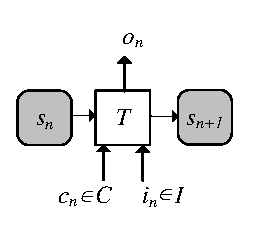
\includegraphics{mealy}
\caption{Mealy finite state machine with configuration}
\label{mealy}
\end{figure}

As shown in Figure \ref{mealy},
as well as in the remainder of this paper,
the state is represented as a gray round corner box,
and the transition function $T$ is represented as a white rectangle.

We denote the configuration letter at the $n$-th cycle as $c_n$.
We further denote the sequence of configuration letter from the $n$-th to the $m$-th cycle as $c_n^m$.

\begin{figure}[b]
\begin{center}
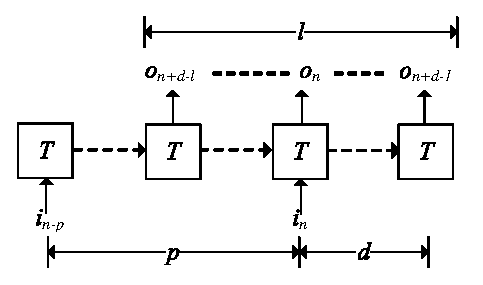
\includegraphics[width=0.45\textwidth]{t1}
\end{center}
\caption{The parameterized complementary condition}
  \label{t1}
\end{figure}

\begin{definition11}\label{def_ass}
\textbf{An assertion(or a formula) on configuration pins} is a configuration letter set $R$.
For a configuration letter $c$,
$R(c)$ means $c\in R$.
If $R(c)$ holds,
we also say that $R$ covers $c$.
\end{definition11}


As shown in Figure \ref{t1},
a sufficient condition for the existence of $E^{-1}$ is,
there exist three parameters $p$, $d$ and $l$,
so that $i_n$ of $E$ can be uniquely determined by the output sequence $o_{n+d-l}^{n+d-1}$.
$d$ is the relative delay between $o_{n+d-l}^{n+d-1}$ and $i_n$,
while $l$ is the length of $o_{n+d-l}^{n+d-1}$,
and $p$ is the length of the prefix path used to rule out some unreachable states.
This condition is formally defined below:

\begin{definition11}\label{def_pcc}%\addtolength{\itemsep}{-0.5\baselineskip}
%{\setlength{\baselineskip}{0.5\baselineskip}
\textbf{Parameterized Complementary Condition (PC)}:
For encoder $E$,
assertion $R$,
and three integers $p$,$d$ and $l$,
$E\vDash PC(p,d,l,R)$ holds if
\begin{enumerate}
 \item $i_n$ can be uniquely determined by $o_{n+d-l}^{n+d-1}$ on $s_{n-p}^{n+d-1}$.
 \item The assertion $R$ covers all $c_x$, where $n-p\le x\le n+d-1$.
\end{enumerate}

This equals the unsatisfiability of $F_{PC}(p,d,l,R)$ in Equation (\ref{uniqt1}).
We further define $E\vDash PC(R)$ as $\exists p,d,l:E\vDash PC(p,d,l,R)$.
\end{definition11}

\begin{equation}\label{uniqt1}
\begin{split}
&F_{PC}(p,d,l,R)\stackrel{def}{=}\\
&\left\{
\begin{array}{cc}
&\bigwedge_{m=n-p}^{n+d-1}
\{
(s_{m+1},o_m)\equiv T(s_m,i_m,c_m)
\}
\\
\wedge&\bigwedge_{m=n-p}^{n+d-1}
\{
(s'_{m+1},o'_m)\equiv T(s'_m,i'_m,c'_m)
\}
\\
\wedge&\bigwedge_{m=n+d-l}^{n+d-1}o_m\equiv o'_m \\
\wedge& i_n\ne i'_n \\
\wedge&\bigwedge_{x=n-p}^{n+d-1}c_x\equiv c \\
\wedge&\bigwedge_{x=n-p}^{n+d-1}c_x'\equiv c \\
\wedge& R(c)
\end{array}
\right\}
\end{split}
\end{equation}

%This definition is the same as that of Subsection \ref{subsec_chkextdec} and paper \cite{ShengYuShen:iccad09}.

The 2nd to 5th lines of Equation (\ref{uniqt1}) correspond to Condition 1 of Definition \ref{def_pcc}.
The 2nd and the 3rd lines of Equation (\ref{uniqt1}) correspond respectively to two paths of $E$.
The only difference between them is that a prime is appended to every variable in the 3rd line.
The 4th line forces the output sequences of these two paths to be the same,
while the 5th line forces their input letters to be different.

At the same time,
the last three lines of Equation (\ref{uniqt1}) correspond to Condition 2 of Definition \ref{def_pcc}.
The 6th and the 7th lines constrain that all configuration letters are equal to $c$,
while the last line constrains $c$ to be covered by $R$.

The algorithm based on checking $E\vDash PC(R)$\cite{ShengYuShen:iccad09,ShengYuShen:tcad} just enumerates all combinations of $p$,$d$ and $l$,
from small to large,
until $F_{PC}(p,d,l,R)$ becomes unsatisfiable,
which means that the decoder $E^{-1}$ exists.

\begin{figure}[b]
\begin{center}
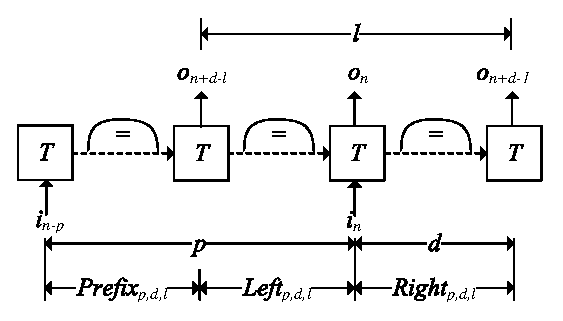
\includegraphics[width=0.45\textwidth]{doubleloop}
\end{center}
\caption{The loop-like non-complementary condition}
  \label{fig_double_loop}
\end{figure}

\section{A Halting Algorithm to Infer Assertion}\label{sec_exist}
$PC$ in Definition \ref{def_pcc} only defines how to determine the existence of decoder $E^{-1}$.
So when the decoder does not exist,
the algorithm based on checking $E\vDash PC(R)$\cite{ShengYuShen:iccad09,ShengYuShen:tcad} will never halt.

To find a halting algorithm,
we must define how to determine the non-existence of $E^{-1}$.
This will be discussed in subsection \ref{subsec_chknonext},
while the proof of its correctness is presented in subsection \ref{subsec_correctness}.
Based on this result,
the overall framework of our algorithm will be presented in subsection \ref{subsec_algo},

\subsection{Determining the non-existence of the decoder}\label{subsec_chknonext}


According to Definition \ref{def_pcc} and Figure \ref{t1},
$E^{-1}$ exists if there is a parameter value tuple $<p,d,l>$ that makes
$E\vDash PC(p,d,l,R)$ holds.
% such that every path longer than $p$ always reaches a particular state $s_n$,
% in which the input letter $i_n$ can be uniquely determined by the output sequence $o_{n+d-l}^{n+d-1}$.

So,
intuitively,
$E^{-1}$ does not exist if for every parameter value tuple $<p,d,l>$,
we can always find another tuple $<p',d',l'>$ with $p'>p$,$l'>l$ and $d'>d$,
such that $E\vDash PC(p',d',l',R)$ does not hold.

This case can be detected by the SAT instance in Figure \ref{fig_double_loop},
which is similar to Figure \ref{t1},
except that three new constraints are inserted to detect loops on paths $s_{n-p}^{n+d-l}$,$s_{n+d-l+1}^n$ and $s_{n+1}^{n+d}$.


\begin{figure}[t]
\begin{center}
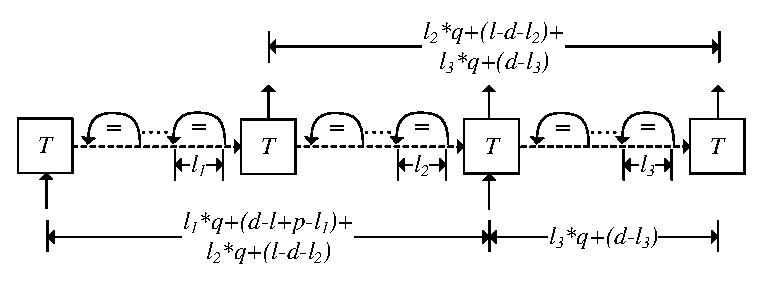
\includegraphics[width=0.45\textwidth]{doubleloop_unfold}
\end{center}
\caption{The loop-like non-complementary condition unfolded for $q$ times}
  \label{fig_double_loop_unfold}
\end{figure}

If this SAT instance is satisfiable,
for any parameter value $<p,d,l>$,
we can unfold these three loops until we find $<p',d',l'>$ that is larger than $<p,d,l>$.
We will prove in next subsection that this unfolded instance is still satisfiable,
which means $E\vDash PC(p',d',l',R)$ does not hold.
So the decoder does not exist.

According to Line 2 and 3 of Equation (\ref{uniqt1}),
there are actually two paths,
so we need to detect these loops on both of them,
i.e.,
on the product machine $M^2$ defined below:

\begin{definition11}%\addtolength{\itemsep}{-0.5\baselineskip}
%{\setlength{\baselineskip}{0.5\baselineskip}
\textbf{Product machine:} For Mealy machine $M=(S,s_0,I,C,O,T)$,
its product machine is $M^2=(S^2,s_0^2,I^2,C^2$ $,O^2,T^2)$,
where
$T^2$ is defined as $(<s_{m+1},s'_{m+1}>,<o_m,o'_m>)=T^2(<s_m,s'_m>,<i_m,i'_m>,<c_m,c'_m>)$ with $(s_{m+1},o_m)=T(s_m,i_m,c_m)$ and $(s'_{m+1},o'_m)=T(s'_m,i'_m,c'_m)$.
\end{definition11}

Thus,
we define the loop-like non-complementary condition below to determine the non-existence of $E^{-1}$:

\begin{definition11}\label{def_lnc}%\addtolength{\itemsep}{-0.5\baselineskip}
%{\setlength{\baselineskip}{0.5\baselineskip}
\textbf{Loop-like Non-complementary Condition (LN):} For encoder $E$ and its Mealy machine $M=(S,s_0,I,C,O,T)$,
assume its product machine is $M^2=(S^2,s_0^2$ $,I^2,C^2,O^2,T^2)$,
then $E\vDash LN(p,d,l,R)$ holds if
$i_n$ can not be uniquely determined by $o_{n+d-l}^{n+d-1}$ on the path $s_{n-p}^{n+d-1}$,
and there are loops on $(s^2)_{n-p}^{n+d-l}$, $(s^2)_{n+d-l+1}^n$ and $(s^2)_{n+1}^{n+d}$.
This equals the satisfiability of $F_{LN}(p,d,l,R)$ in Equation (\ref{uniqln}).
We further define $E\vDash LN(R)$ as $\exists p,d,l:E\vDash LN(p,d,l,R)$.
\end{definition11}


\begin{equation}\label{uniqln}
\begin{split}
&F_{LN}(p,d,l,R)\stackrel{def}{=}\\
&\left\{
\begin{array}{cc}
&\bigwedge_{m=n-p}^{n+d-1}
\{
(s_{m+1},o_m)\equiv T(s_m,i_m,c_m)
\}
\\
\wedge&\bigwedge_{m=n-p}^{n+d-1}
\{
(s'_{m+1},o'_m)\equiv T(s'_m,i'_m,c'_m)
\}
\\
\wedge&\bigwedge_{m=n+d-l}^{n+d-1}o_m\equiv o'_m \\
\wedge& i_n\ne i'_n \\
\wedge&\bigwedge_{x=n-p}^{n+d-1}c_x\equiv c \\
\wedge&\bigwedge_{x=n-p}^{n+d-1}c_x'\equiv c \\
\wedge& R(c) \\
\wedge& \bigvee_{x=n-p}^{n+d-l-1}\bigvee_{y=x+1}^{n+d-l} \{s_x\equiv s_y\wedge s'_x\equiv s'_y\} \\
\wedge& \bigvee_{x=n+d-l+1}^{n-1}\bigvee_{y=x+1}^{n} \{s_x\equiv s_y\wedge s'_x\equiv s'_y\} \\
\wedge& \bigvee_{x=n+1}^{n+d-1}\bigvee_{y=x+1}^{n+d} \{s_x\equiv s_y\wedge s'_x\equiv s'_y\}
\end{array}
\right\}
\end{split}
\end{equation}

By comparing Equation (\ref{uniqt1}) and (\ref{uniqln}),
it is obvious that their only difference lies in the last three newly inserted lines in (\ref{uniqln}),
which will be used to detect loops on the following three paths shown in Figure \ref{fig_double_loop}:
\begin{equation}
\begin{array}{c}
Prefix_{p,d,l}=(s^2)_{n-p}^{n+d-l} \\
Left_{p,d,l}=(s^2)_{n+d-l+1}^n \\
Right_{p,d,l}=(s^2)_{n+1}^{n+d}
\end{array}
\end{equation}

In the next subsection,
we will prove that $E\vDash LN(R)\leftrightarrow \neg \{E\vDash PC(R)\}$,
that is,
$LN$ and $PC$ are exclusive to each other.



Before proceeding to next subsection,
we need to define how to unfold these loops in above three paths.
Assume that the length of loops in $Prefix_{p,d,l}$, $Left_{p,d,l}$ and $Right_{p,d,l}$ are $l_1$, $l_2$ and $l_3$ respectively.
We further assume that we unfold these loops for $q$ times.
Then,
the SAT instance generated from this unfolding is shown in Figure \ref{fig_double_loop_unfold},
It is obvious that,
the unfolded SAT instance corresponds to $F_{LN}(p",d",l",R)$,
where:

\begin{equation}
\begin{array}{ccc}
p"&=&l_1*q+(d-l+p-l_1)+l_2*q+(l-d-l_2) \\
d"&=&l_3*q+(d-l_3) \\
l"&=&l_2*q+(l-d-l_2)+l_3*q+(d-l_3)
\end{array}
\end{equation}

It is obvious that for every particular $<p,d,l>$ and $<p',d',l'>$,
there always exists a $q$,
such that $Prefix_{p",d",l"}$, $Left_{p",d",l"}$ and $Right_{p",d",l"}$ resulted from this unfolding
are \textbf{not shorter} than $Prefix_{p',d',l'}$,$Left_{p',d',l'}$ and $Right_{p',d',l'}$ respectively.



\subsection{Proving correctness}\label{subsec_correctness}

Before proving $E\vDash LN(R)\leftrightarrow \neg \{E\vDash PC(R)\}$,
we need some lemmas.

\begin{figure}[b]
\centering
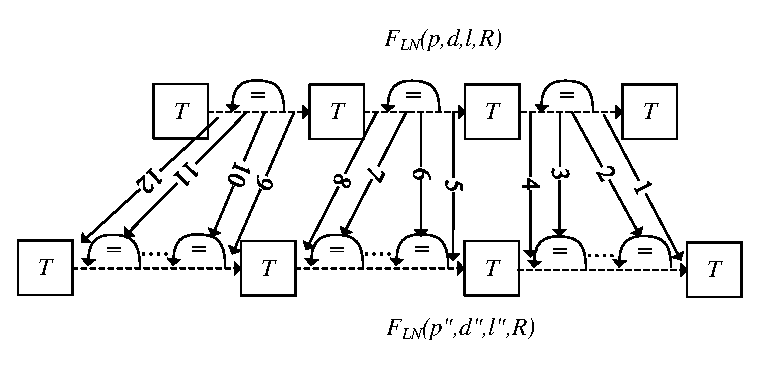
\includegraphics[width=0.45\textwidth]{doubleloop_unfold_cmp}
\caption{Correspondance between $F_{LN}(p,d,l,R)$ and $F_{LN}(p",d",l",R)$}
\label{doubleloop_unfold_cmp}
\end{figure}

\begin{lemma}[]\label{lemma_unfold_longer}
For $F_{LN}(p",d",l",R)$ in Figure \ref{fig_double_loop_unfold},
we have $F_{LN}(p,d,l,R)\to F_{LN}(p",d",l",R)$
\end{lemma}
\begin{proof}
The formula $F_{LN}(p",d",l",R)$ is:

\begin{equation}\label{equ_correspondance}
\begin{split}
&F_{LN}(p",d",l",R)\stackrel{def}{=}\\
&\left\{
\begin{array}{cc}
&\bigwedge_{m=n-p"}^{n+d"-1}
\{
(s_{m+1},o_m)\equiv T(s_m,i_m,c_m)
\}
\\
\wedge&\bigwedge_{m=n-p"}^{n+d"-1}
\{
(s'_{m+1},o'_m)\equiv T(s'_m,i'_m,c'_m)
\}
\\
\wedge&\bigwedge_{m=n+d"-l"}^{n+d"-1}o_m\equiv o'_m \\
\wedge& i_n\ne i'_n \\
\wedge&\bigwedge_{x=n-p"}^{n+d"-1}c_x\equiv c \\
\wedge&\bigwedge_{x=n-p"}^{n+d"-1}c_x'\equiv c \\
\wedge& R(c) \\
\wedge& \bigvee_{x=n-p"}^{n+d"-l"-1}\bigvee_{y=x+1}^{n+d"-l"} \{s_x\equiv s_y\wedge s'_x\equiv s'_y\} \\
\wedge& \bigvee_{x=n+d"-l"+1}^{n-1}\bigvee_{y=x+1}^{n} \{s_x\equiv s_y\wedge s'_x\equiv s'_y\} \\
\wedge& \bigvee_{x=n+1}^{n+d"-1}\bigvee_{y=x+1}^{n+d"} \{s_x\equiv s_y\wedge s'_x\equiv s'_y\}
\end{array}
\right\}
\end{split}
\end{equation}

Assume that $F_{LN}(p,d,l,R)$ is satisfied,
and its satisfying assignment is $A$.
We need to prove that $F_{LN}(p",d",l",R)$ is also satisfied with $A$.

The directed arcs numbered from 1 to 12 in Figure \ref{doubleloop_unfold_cmp},
show the correspondence between $F_{LN}(p,d,l,R)$ and the $F_{LN}(p",d",l",R)$.

The arcs 2 and 3 mean that we can apply the satisfying assignment of the loop in $Right_{p,d,l}$
to the unfolded loops in $Right_{p",d",l"}$.
The arcs 1 and 4 mean that we can apply the the satisfying assignments of the two paths not in the loop,
to $Right_{p",d",l"}$.
With the arcs from 1 to 4,
we can make the path $Right_{p",d",l"}$ satisfiable.

Similarly,
we can also make the paths $Prefix_{p",d",l"}$ and $Left_{p",d",l"}$ satisfiable.

Thus the 2nd line of Equation (\ref{equ_correspondance}) is satisfied with the assignment $A$.

Similarly,
the 3rd to 8th lines of Equation (\ref{equ_correspondance}) are also satisfied with the assignment $A$.

At the same time,
there are $q$ loops in $Prefix_{p",d",l"}$, $Left_{p",d",l"}$ and $Right_{p",d",l"}$,
which will make the last three lines in Equation (\ref{equ_correspondance}) satisfied.

Thus,the satisfying assignment $A$ of $F_{LN}(p,d,l,R)$ can also make $F_{LN}(p",d",l",R)$ satisfied.

This concludes the proof.
\end{proof}

\begin{lemma}[]\label{lemma_pc_long}
For two tuples $<p,d,l>$ and $<p',d',l'>$,
if $Prefix_{p',d',l'}$,$Left_{p',d',l'}$ and $Right_{p',d',l'}$ are \textbf{not shorter} than $Prefix_{p,d,l}$,$Left_{p,d,l}$ and $Right_{p,d,l}$ respectively,
then $E\vDash PC(p,d,l,R)\to E\vDash PC(p',d',l',R)$.
\end{lemma}
\begin{proof}
It is obvious that $F_{PC}(p,d,l,R)$ is a sub-formula of $F_{PC}(p',d',l',R)$,
so the unsatisfiability of the former implies the unsatisfiability of the latter.
Thus,
$E\vDash PC(p,d,l,R)\to E\vDash PC(p',d',l',R)$ holds.
\end{proof}

The following two theorems will prove that $E\vDash LN(R)\leftrightarrow \neg \{E\vDash PC(R)\}$.

\begin{theorem}[]\label{thm_pc_nln}
$E\vDash LN(R)\to \neg \{E\vDash PC(R)\}$
\end{theorem}
\begin{proof}
We can prove it by contradiction.
Assume that $E\vDash LN(R)$ and $E\vDash PC(R)$ both hold.
This means there exist $<p,d,l>$ and $<p',d',l'>$,
such that $E\vDash PC(p,d,l,R)$ and $E\vDash LN(p',d',l',R)$.

On one hand,
$E\vDash LN(p',d',l',R)$ implies that there are loops in the paths $Prefix_{p',d',l'}$,$Left_{p',d',l'}$ and $Right_{p',d',l'}$.
By unfolding these loops,
we can get another tuple $<p",d",l">$,
so that :
\begin{enumerate}
\item $Prefix_{p",d",l"}$,$Left_{p",d",l"}$ and $Right_{p",d",l"}$ are longer than $Prefix_{p,d,l}$,$Left_{p,d,l}$ and $Right_{p,d,l}$ respectively
\item According to Lemma \ref{lemma_unfold_longer},
$F_{LN}(p",d",l",R)$ is satisfiable.
\end{enumerate}

$F_{PC}(p",d",l",R)$ is a sub-formula of $F_{LN}(p",d",l",R)$,
so $F_{PC}(p",d",l",R)$ is also satisfiable,
which means that $E\vDash PC(p",d",l",R)$ does not hold.

On the other hand,
according to Lemma \ref{lemma_pc_long},
$E\vDash PC(p",d",l",R)$ holds.

This contradiction concludes the proof.
\end{proof}

\begin{theorem}[]\label{thm_nln_pc}
$E\vDash LN(R)\gets \neg \{E\vDash PC(R)\}$
\end{theorem}
\begin{proof}
We can also prove it by contradiction.
Assume that neither $E\vDash LN(R)$ nor $E\vDash PC(R)$ holds.
Then for every $<p,d,l>$ and $<p',d',l'>$,
$F_{PC}(p,d,l,R)$ is satisfiable,
while $F_{LN}(p',d',l',R)$ is unsatisfiable.

Thus,
assume $uirrd(M^2)$ is the uninitialized state variables recurrence diameter of $E$'s product machine.
Let's define $<p,d,l>$ as:
\begin{equation}
\begin{array}{c}
p=uirrd(M^2)*2+2 \\
d=uirrd(M^2)+1 \\
l=uirrd(M^2)*2+2
\end{array}
\end{equation}

With this definition,
it is obvious that $Prefix_{p,d,l}$,$Left_{p,d,l}$ and $Right_{p,d,l}$ are all longer than $uirrd(M^2)$.
This means there are loops in all these three paths,
which will make $F_{LN}(p,d,l,R)$ satisfiable.
This contradicts with the fact that $F_{LN}(p',d',l',R)$ is unsatisfiable for every $<p',d',l'>$.

This contradiction concludes the proof.
\end{proof}


\subsection{Algorithm implementation}\label{subsec_algo}
Theorems \ref{thm_pc_nln} and \ref{thm_nln_pc} show that,
we can enumerate all combinations of $<p,d,l>$ from small to large,
and check $E\vDash PC(p,d,l,R)$ and $E\vDash LN(p,d,l,R)$ in every iteration.
This process will eventually terminate with one and only one answer between $E\vDash PC(R)$ and $E\vDash LN(R)$.
The implementation of this algorithm will be presented below.

\begin{algorithm}
\caption{InferAssertion}
\label{algo_pcln}
\begin{algorithmic}[1]
\STATE $NA=\{\}$
\FOR{$x=0\to \infty$}
\STATE $<p,d,l>=<2x,x,2x>$
\IF{$F_{PC}(p,d,l,\bigwedge_{na\in NA}\neg na)$ is unsatisfiable}
\IF{$\bigwedge_{na\in NA}\neg na$ is satisfiable}
\STATE decoder exists with final assertion $\bigwedge_{na\in NA}\neg na$
\ELSE
\STATE decoder does not exist
\ENDIF
\STATE halt
\ELSIF{$F_{LN}(p,d,l,\bigwedge_{na\in NA}\neg na)$ is satisfiable}
\STATE let $c$ be the configuration letter leading to the non-existence of decoder
\STATE $na\leftarrow InferCoveringFormula(c)$
\STATE $NA\leftarrow NA\cup \{na\}$
\ENDIF
\ENDFOR
\end{algorithmic}
\end{algorithm}

In Line 1 of Algorithm \ref{algo_pcln},
$NA$ will be used to record all inferred formulas that can lead to the non-existence of the decoder.
They are all inferred by the procedure $InferCovering$ $Formula$ in Line 13,
whose functionality is to infer a formula that can cover not only $c$,
but also many other configuration letters leading to the non-existence of the decoder.
More details of this procedure will be presented in Section \ref{sec_infer}.

Line 3 ensures that the length of $Prefix_{p,d,l}$,$Left_{p,d,l}$ and $Right_{p,d,l}$ are all set to $x$,
whose value is enumerated in Line 2.
In this way,
many redundant combinations of $p$,$d$ and $l$ are no longer need to be tested.
Thus, the performance of this algorithm can be significantly boosted.

Line 4 means the input letter can be uniquely determined by the output sequence with the assertion $\bigwedge_{na\in NA}\neg na$.
Line 5 means that there is at least one configuration letter that can lead to the existence of the decoder,
and the final assertion is created by anding all inverses of $NA$ assertions in the 6th line.

Line 7 means that the inferred assertion $\bigwedge_{na\in NA}\neg na$ has ruled out all configuration letters,
that is,
no configuration letter can lead to the existence of the decoder.
There must be some bugs in the encoder.

Line 11 means that the decoder does not exist with the configuration letter $c$ in Line 12.
We need to rule out $c$ such that Algorithm \ref{algo_pcln} can continue searching for other configuration letters that may lead to the existence of the decoder.
The procedure $InferCoveringFormula$ in Line 13 will be used to infer a formula $na$ that covers not only $c$,
but also a large set of invalid configuration letters.
They will be ruled out in Line 14.

We can prove that Algorithm \ref{algo_pcln} is a halting one.
\begin{theorem}[]\label{thm_pcln_halt}
Algorithm \ref{algo_pcln} is a halting algorithm.
\end{theorem}
\begin{proof}
According to Theorems \ref{thm_pc_nln} and \ref{thm_nln_pc},
Algorithm \ref{algo_pcln} will eventually reach Line 4 or 11.

In the former case,
this algorithm will halt at Line 10.

In the latter case,
a new formula $na$ will be inferred,
which will cover the configuration letter $c$.
Because the number of such $c$ is finite,
all of them will eventually be ruled out by $\bigwedge_{na\in NA}\neg na$.
Then Algorithm \ref{algo_pcln} will eventually reach Line 4,
and halt at Line 10.

\end{proof}

\section{Inferring New Formula Covering Invalid Configuration Letter $c$}\label{sec_infer}
This section will introduce the implementation of $InferC$ $overingFormula$ in Line 13 of Algorithm \ref{algo_pcln}.
It will be used to infer a Boolean formula $na$
that covers not only $c$,
but also many other configuration letters leading to the non-existence of the decoder.
This job will be accomplished in the following three steps:
\begin{enumerate}
 \item Transforming $F_{LN}$ into an equivalent form with an object variable,
       such that it can be used to defined a Boolean function $f$.
 \item Eliminating some variables from the support set of $f$ with cofactoring\cite{Cofact},
       until only $c$ remains.
 \item Characterizing $f$ with Craig Interpolation.
       This $f$ is also the formula $na$ in Line 13 of Algorithm \ref{algo_pcln}.
\end{enumerate}

These three steps will be presented in the following three subsections.

\subsection{An equivalent form of $F_{LN}$}

As mentioned above,
we need to transform $F_{LN}$ into another equivalent form with an object variable.

First,
we need to move the 4th line and the last three lines of Equation (\ref{uniqln}) into a new subformula:

\begin{equation}\label{uniqln_subg}
\begin{split}
&G(p,d,l)\stackrel{def}{=}\\
&\left\{
\begin{array}{cc}
&\bigwedge_{m=n+d-l}^{n+d-1}o_m\equiv o'_m \\
\wedge& \bigvee_{x=n-p}^{n+d-l-1}\bigvee_{y=x+1}^{n+d-l} \{s_x\equiv s_y\wedge s'_x\equiv s'_y\} \\
\wedge& \bigvee_{x=n+d-l+1}^{n-1}\bigvee_{y=x+1}^{n} \{s_x\equiv s_y\wedge s'_x\equiv s'_y\} \\
\wedge& \bigvee_{x=n+1}^{n+d-1}\bigvee_{y=x+1}^{n+d} \{s_x\equiv s_y\wedge s'_x\equiv s'_y\}
\end{array}
\right\}
\end{split}
\end{equation}

And then,
$F_{LN}$ can be transformed into :
\begin{equation}\label{uniqln_new}
\begin{split}
&F'_{LN}(p,d,l,R)\stackrel{def}{=}\\
&\left\{
\begin{array}{cc}
&\bigwedge_{m=n-p}^{n+d-1}
\{
(s_{m+1},o_m)\equiv T(s_m,i_m,c_m)
\}
\\
\wedge&\bigwedge_{m=n-p}^{n+d-1}
\{
(s'_{m+1},o'_m)\equiv T(s'_m,i'_m,c'_m)
\}
\\
\wedge& i_n\ne i'_n \\
\wedge&\bigwedge_{x=n-p}^{n+d-1}c_x\equiv c \\
\wedge&\bigwedge_{x=n-p}^{n+d-1}c_x'\equiv c \\
\wedge& R(c) \\
\wedge& t\equiv G(p,d,l)
\end{array}
\right\}
\end{split}
\end{equation}

It is obvious that $F_{LN}$ and $F'_{LN}\wedge t\equiv 1$ is equisatisfiable.

At the same time,
according to Figure \ref{fig_double_loop},
$F'_{LN}$ actually defines a function $f':S^{2}\times I^{(d+p)*2}\times C\to B$,
whose support set $supp(f')$ is $\{s_{n-p},s'_{n-p},i_{n-p}^{n+d-1},(i')_{n-p}^{n+d-1},c\}$,
and its output is the object variable $t$ in the last line of Equation (\ref{uniqln_new}).

\subsection{Cofactoring}
According to Line 11 of Algorithm \ref{algo_pcln},
$F_{LN}$ is satisfiable.
We further assume that $A$ is the satisfying assignment of $F_{LN}$.
We can just assert the value of $i_{n-p}^{n+d-1}$, $(i')_{n-p}^{n+d-1}$, $s_{n-p}$ and $(s')_{n-p}$ into formula $F'_{LN}$,
and get :

\begin{equation}\label{equ_char}
\begin{split}
&F"_{LN}(c,t)\stackrel{def}{=}\\
&\left\{
\begin{array}{cc}
& F'_{LN}\\
\wedge& i_{n-p}^{n+d-1}\equiv A(i_{n-p}^{n+d-1})\\
\wedge& (i')_{n-p}^{n+d-1}\equiv A((i')_{n-p}^{n+d-1})\\
\wedge& s_{n-p}\equiv A(s_{n-p})\\
\wedge& (s')_{n-p}\equiv A((s')_{n-p})
\end{array}
\right\}
\end{split}
\end{equation}

Now,
$F"_{LN}$ defines another function $f"$,
whose support set is reduced to $c$.
It is obvious that $F"_{LN}(c,t)\wedge t\equiv 1$ is already the formula that covers a set of invalid configuration letters.
But it is still a large complicated CNF clause set.
To reduce its size,
we need the characterizing algorithm in the next subsection.

\subsection{Characterizing $f"$ with Craig interpolation}

We then encode $F"_{LN}(c,t)$ into the CNF format,
and denote it as $CNF(F"_{LN}(c,t))$.
Assume $CNF'(F"_{LN}(c,t'))$ is a copy of $CNF(F"_{LN}(c,t))$.
They share the same variable index for $c$ only,
while all other variables are encoded independently.
In this way,
we can construct formula $\phi_A$ and $\phi_B$ as:

\begin{equation}\label{equ_interpA}
\phi_A\stackrel{def}{=}CNF(F"_{LN}(c,t))\wedge t\equiv 1
\end{equation}

\begin{equation}\label{equ_interpB}
\phi_B\stackrel{def}{=}CNF'(F"_{LN}(c,t'))\wedge t'\equiv 0
\end{equation}

It is obvious that $\phi_A\wedge \phi_B$ is unsatisfiable.
With the interpolant generating algorithm proposed by McMillan\cite{interp_McMillan},
we can generate an interpolant,
which is a circuit with Boolean function $ITP:C\to B$.

According to Theorem \ref{thm_craig},
$ITP$ is inconsistent with $\phi_B$ in Equation (\ref{equ_interpB}).
So it characterizes a set $C'\subseteq C$ that can make $\phi_A$ in Equation (\ref{equ_interpA}) satisfiable.
According to Equations (\ref{uniqln_new}) and (\ref{equ_char}),
it is obvious that:
\begin{enumerate}
 \item The $c$ in Line 12 of of Algorithm \ref{algo_pcln} is in $C'$.
According to Theorem \ref{thm_pcln_halt},
this will ensure that Algorithm \ref{algo_pcln} is halting.
 \item All $c'\in C'$ can also lead to the non-existence of the decoder.
This will speedup Algorithm \ref{algo_pcln} significantly.
\end{enumerate}

\section{Removing Redundancy}\label{sec_rmred}
\begin{algorithm}
\caption{$RemoveRedundancy(p,d,l,R)$}
\label{algo_remove}
\begin{algorithmic}[1]
\FOR{$p'=p \to 0$}
  \IF{$F_{PC}(p'-1,d,l,R)$ is satisfiable}
    \STATE break
  \ENDIF
\ENDFOR
\FOR{$d'=d \to 0$}
  \IF{$F_{PC}(p',d'-1,l,R)$ is satisfiable}
    \STATE break
  \ENDIF
\ENDFOR
\FOR{$l'=1 \to l-(d-d')$}
  \IF{$F_{PC}(p',d',l',R)$ is unsatisfiable}
    \STATE break
  \ENDIF
\ENDFOR
\PRINT \texttt{"final result is $<p',d',l'>$"}
\end{algorithmic}
\end{algorithm}

The $<p,d,l>$ found by Algorithm \ref{algo_pcln} contains some redundancy,
which will cause unnecessarily large overheads on the circuit area and the run time of the characterizing Boolean function of the decoder.
So,
Algorithm \ref{algo_remove} is used to minimize $<p,d,l>$ before passing it to the characterization algorithm.

This algorithm just iteratively reduces the value of $p$, $d$ and $l$,
and tests whether the reduced values can still make $E\vDash PC(R)$ holds.
We will not dive into its detail here.


\section{Experimental Results}\label{sec_exp}
We have implemented this algorithm in the OCaml language,
and solved the generated SAT instances with Minisat solver\cite{EXTSAT}.
All experiments are run on a PC with a 2.4GHz Intel Core 2 Q6600 processor, 8GB memory and Ubuntu 10.04 linux.
%All experimental results and programs can be downloaded from \url{http://www.ssypub.org}.
%All related programs and data files can be downloaded from \url{http://www.ssypub.org}.
\subsection{Benchmarks}

\begin{table}[b]
\centering
\caption{Information of Benchmarks}
\begin{tabular}{|c|c|c|c|c|c|}
\hline
&XGXS&XFI&scrambler&PCIE&T2 et-\\
&&&&&hernet\\\hline
Line number&&&&&\\
of Verilog&214&466&24&1139&1073\\
source code&&&&&\\\hline
\#regs&15&135&58&22&48\\\hline
Data path&8&64&66&10&10\\
width&&&&&\\ \hline
\end{tabular}\label{tab_benchmark}
\end{table}




Table \ref{tab_benchmark} shows information of the following benchmarks.
\begin{enumerate}

\item A XGXS encoder compliant to clause 48 of IEEE-802.3ae 2002 standard \cite{IEEE80232002}.

\item A XFI encoder compliant to clause 49 of the same IEEE standard.

\item A 66-bit scrambler used to ensure
that a data sequence has sufficiently many 0-1 transitions,
so that it can run through a high-speed
noisy serial transmission channel.

\item A PCI-E physical coding module \cite{PCIESPEC}.

\item The Ethernet module of Sun's OpenSparc T2 processor.
\end{enumerate}

\subsection{Results}
\begin{table}[t]
\centering
\caption{Experimental Results}
\begin{tabular}{|c|c|c|c|c|c|c|}
\hline
&                                        &XG-     &XFI       &scra-     &PCI-    &T2 e-\\
&                                        &XS      &          &mbler     &E         &ther\\\hline
&Run time                           &&&&&\\
&checking                    &0.07     &17.84     &2.70      &0.47    &30.59       \\
\cite{ShengYuShen:fmcad10}&$PC$(sec)     &&&&&\\\cline{2-7}
&$d,p,l$                                 &1,2,1    &0,3,2     &0,2,2     &2,2,1   &4,2,1         \\ \hline\hline
&Config                 &&&&&\\
&pin number                              &3        &120       &1         &16      &26\\\cline{2-7}
&Run time                         &&&&&\\
ours&inferring                   &3.69     &372.15    &3.14      &30.53   &188.56      \\
&assertion                      &&&&&\\\cline{2-7}
&$d,p,l$                                 &1,3,1    &0,4,2     &0,2,2     &2,2,1   &4,4,1          \\ \hline
\end{tabular}\label{tab_res}
\end{table}

The 2nd row of Table \ref{tab_res} shows the run time of checking the decoder's existence
with the other halting algorithm proposed previously by Shen et.al\cite{ShengYuShen:fmcad10}.
And the 3rd row shows the value of $d$, $p$ and $l$ discovered by that algorithm.

At the same time,
the 4th row shows the configuration pin's bit number,
the 5th row shows the run time of inferring assertion with our new algorithm,
while the last line shows the value of $d$, $p$ and $l$ discovered.

By comparing the 2nd and the 5th rows,
it is obvious that our approach is much slower than that of \cite{ShengYuShen:fmcad10},
which is caused by the much more complicated procedure $InferCove$ $ringFormula$
used to infer new formulas.

By comparing the 3rd and the 6th rows,
it is obvious that there are some minor differences on those parameter values.
This is caused by the different orders in checking various parameter combinations.

\subsection{Inferred assertions}
We will show here the inferred assertions.

\textbf{For XGXS}:

!( ( bad\_disp \& !rst \& bad\_code ) ) \& !( ( rst \& bad\_code ) ) \& !( ( !rst \& !bad\_disp \& bad\_code ) )

\textbf{For XFI}:

!( ( !RESET \& !TEST\_MODE \& !DATA\_VALID \& DATA \_PAT\_SEL ) ) \& !( ( !RESET \& !TEST\_MODE \& !DATA\_VA LID \& !DATA\_PAT\_SEL ) )

\textbf{For scrambler}:

True

\textbf{For PCI-E}:

!( ( CNTL\_RESETN\_P0 \& !TXELECIDLE \& CNTL\_TXE nable\_P0 \& CNTL\_Loopback\_P0 ) | ( CNTL\_RESETN\_P0 \& !TXELECIDLE \& !CNTL\_TXEnable\_P0 ) ) \& !( ( CNTL\_RE SETN\_P0 \& TXELECIDLE ) | ( CNTL\_RESETN\_P0 \& !TXELECIDLE \& !CNTL\_TXEnable\_P0 ) | ( !CNTL\_RESET N\_P0 ) )

\textbf{For T2 ethernet}:

!( ( reset\_tx \& !txd\_sel[0] \& !txd\_sel[1] \& link\_up\_loc \& jitter\_study\_pci[0] \& !jitter\_study\_pci[1] ) ) \& !( ( reset\_tx \& !txd\_sel[0] \& !txd\_sel[1] \& link\_up\_loc \& jitter\_study\_pci[0] \& jitter\_study\_pci[1] ) ) \& !( ( reset\_tx \& !txd\_sel[0] \& !txd\_sel[1] \& link\_up\_loc \& !jitter\_study\_pci[0] \& jitter\_study\_pci[1] ) ) \& !( ( jitter\_study\_pci[1] \& jitter\_study\_pci[0] \& !txd\_sel[0] \& !txd\_sel[1] \& !reset\_tx \& link\_up\_loc ) ) \& !( ( jitter\_study\_pci[1] \& !jitter\_study\_pci[0] \& !reset\_tx \& !txd\_sel[0] \& !txd\_sel[1] \& link\_up\_loc ) ) \& !( ( jitter\_study\_pci[0] \& !jitter\_study\_pci[1] \& !txd\_sel[0] \& !txd\_sel[1] \& !reset\_tx \& link\_up\_loc ) ) \& !( ( reset\_tx \& !jitter\_study\_pci[0] \& !txd\_sel[0] \& !txd\_sel[1] \& link\_up\_loc \& !jitter\_study\_pci[1] ) )

% \subsection{Scalability of Our Algorithm}\label{subsec_scale}
% According to the 3th and 6th row,
% the values of $d$, $p$ and $l$ are all small.
% To show that our algorithm can scale to larger parameter values,
% we insert a test logic module into the most complex XFI circuit.
% This module include an eight bit counter,
% which means that its diameter will not be shorter than 256.
% So,
% to infer an assertion that rules out the test mode,
% we need to construct an SAT instance as long as $p+d+1$,
% that is,
% 513.

% We run our algorithm on XFI again.

\section{Related Work}\label{sec_relwork}
\subsection{Complementary synthesis and program inversion}
The concept of complementary synthesis was first proposed by Shen et.al\cite{ShengYuShen:iccad09,ShengYuShen:tcad}.
Its major shortcomings is that it is not halting.
Shen et.al\cite{ShengYuShen:fmcad10} addressed this problem by building a set of over-approximations that is similar to onion-rings.

According to Gulwani\cite{dim_syn},
program inversion is the problem that derive a program $P^{-1}$
that negate the computation of a given program $P$.
So the definition of program inversion is very similar to complementary synthesis.

Initial work on deriving program inversion used proof-based approaches\cite{prog_inv},
but it can only handle very small programs and very simple syntax structures.

Gl\"{u}ck et.al \cite{mtd_autoProginv} inverts the first-order functional programs
by eliminating nondeterminism with LR-based parsing methods.
The requirement that the program to be inverted should be expressed in functional language makes it impossible to apply it to our application.

Srivastava et.al \cite{prog_inv_rev} assumes that an inverted program is typically related to the original program,
so the space of possible inversion can be inferred by automatically
mining the original program for expressions, predicates, and control flow.
This algorithm inductively rules out invalid paths that can't fulfill the requirement of inversion,
to narrow down the space of candidate programs until only the valid ones remain.
So it can only guarantee the existence of a solution,
but not the correctness of this solution if its assumptions do not hold.


\subsection{Protocol converter synthesis}
The protocol converter synthesis is the problem that automatically generates a translator between two different communication protocols.

Avnit et.al \cite{converter_date08} first defines a general model for describing the different protocols.
Then it provides an algorithm to decide
whether there are some functionality of a protocol that can't be translated into another.
Finally,
it synthesizes the translator by computing a greatest fixed point for the update function of buffer's control states.
Avnit et.al\cite{converter_date09} improved the algorithm mentioned above with a more efficient design space exploration algorithm.
%The implementation of this tool is introduced in \cite{converter_tacas10}.

\section{Conclusions}\label{sec_conclude}

This paper proposes a fully automatic approach to infer assertion for complementary synthesis.
Experimental results show that our approach can infer assertions for many complex encoders,
such as PCI-E\cite{PCIESPEC} and Ethernet\cite{IEEE80232002},.

% One direction for future work is to develop an abstraction and refinement framework for complementary synthesis,
% to conquer the very large diameter problem raises in Subsection \ref{subsec_scale}.


%ACKNOWLEDGMENTS are optional
%\section{Acknowledgments}
%This project 60603088 is supported by National Natural Science Foundation of China ,
%and Supported by the Program for Changjiang Scholars and Innovative Research Team in University No IRT0614.
%Thanks to anonymous reviewers for their effort in reviewing this paper.

%This section is optional; it is a location for you
%to acknowledge grants, funding, editing assistance and
%what have you.  In the present case, for example, the
%authors would like to thank Gerald Murray of ACM for
%his help in codifying this \textit{Author's Guide}
%and the \textbf{.cls} and \textbf{.tex} files that it describes.

%
% The following two commands are all you need in the
% initial runs of your .tex file to
% produce the bibliography for the citations in your paper.
\bibliographystyle{abbrv}
%\bibliography{sigproc}  % sigproc.bib is the name of the Bibliography in this case
% You must have a proper ".bib" file
%  and remember to run:
% latex bibtex latex latex
% to resolve all references
%
% ACM needs 'a single self-contained file'!
%


\begin{thebibliography}{10}

\bibitem{ShengYuShen:iccad09}
S.~Shen, J.~Zhang, Y.~Qin, and S.~Li.
\newblock Synthesizing complementary circuits automatically.
\newblock In {\em ICCAD09 Conference Proceedings}, pages 381--388. IEEE,
  November 2009.

\bibitem{ShengYuShen:tcad}
S.~Shen, Y.~Qin, K.~Wang, L.~Xiao, J.~Zhang, and S.~Li.
\newblock Synthesizing complementary circuits automatically.
\newblock {\em IEEE transaction on CAD of Integrated Circuits and Systems},
  29(8):1191--1202, August 2010.

\bibitem{Cofact}
M.~K. Ganai, A.~Gupta, and P.~Ashar.
\newblock Efficient sat-based unbounded symbolic model checking using circuit
  cofactoring.
\newblock In {\em ICCAD04 Conference Proceedings}, pages 510--517. IEEE,
  November 2004.

\bibitem{Craig}
W.~Craig.
\newblock Linear reasoning: A new form of the herbrand-gentzen theorem.
\newblock {\em J. Symbolic Logic}, 22(3):250--268, 1957.

\bibitem{CHAFF}
M. W. Moskewicz, C. F. Madigan, Y. Zhao, L. Zhang, and S. Malik.
\newblock Chaff: Engineering an Efficient SAT Solver.
\newblock In {\em DAC01 Conference Proceedings}, pages 530--535. IEEE, June
  2001.

\bibitem{grasp}
J. P. M. Silva and K. A. Sakallah.
\newblock GRASP - a new search algorithm for satisfiability.
\newblock In {\em ICCAD96 Conference Proceedings}, pages 220--227. IEEE, November
  1996.

\bibitem{BERKMIN}
E. Goldberg and Y. Novikov.
\newblock BerkMin: a fast and robust SAT-solver.
\newblock In {\em DATE02 Conference Proceedings}, pages 142--149. IEEE, March
  2002.

\bibitem{EXTSAT}
N.~E\'en and N.~S\"orensson.
\newblock An extensible sat-solver.
\newblock In {\em SAT03 Conference Proceedings}, pages 502--518. Springer, May
  2003.

\bibitem{PCIESPEC}
{\em PCI Express Base Specification Revision 1.0. Download from
  http://www.pcisig.com}.

\bibitem{IEEE80232002}
{\em IEEE Standard for Information technology Telecommunications and
  information exchange between systems Local and metropolitan area networks
  Specific requirements Part 3: Carrier Sense Multiple Access with Collision
  Detection (CSMA/CD) Access Method and Physical Layer Specifications
  Amendment: Media Access Control (MAC) Parameters, Physical Layers, and
  Management Parameters for 10 Gb/s Operation, IEEE Std. 802.3, 2002.}

\bibitem{interp_McMillan}
K.~L. McMillan.
\newblock Interpolation and sat-based model checking.
\newblock In {\em CAV03 Conference Proceedings}, pages 1--13. Springer, July
  2003.

\bibitem{MEALY}
G.~H. Mealy.
\newblock A method for synthesizing sequential circuits.
\newblock {\em Bell Systems Technical Journal}, 34(5):1045--1079, 1955.

\bibitem{RecDiam}
D.~Kroening and O.~Strichman.
\newblock Efficient computation of recurrence diameters.
\newblock In {\em VMCAI03 Conference Proceedings}, pages 298--309. Springer,
  January 2003.

\bibitem{ShengYuShen:fmcad10}
S.~Shen, Y.~Qin, J.~Zhang, and S.~Li.
\newblock A halting algorithm to determine the existence of decoder.
\newblock In {\em FMCAD10 Conference Proceedings}, pages 91--100. IEEE, October
  2010.

\bibitem{dim_syn}
S.~Gulwani.
\newblock Dimensions in program synthesis.
\newblock In {\em PPDP10 Conference Proceedings}, pages 13--24. ACM, July 2010.

\bibitem{prog_inv}
E.~W. Dijkstra.
\newblock Program inversion.
\newblock In {\em Program Construction 1978 Conference Proceedings}, pages
  54--57, 1978.

\bibitem{mtd_autoProginv}
R.~Gl\"uck and M.~Kawabe.
\newblock A method for automatic program inversion based on lr(0) parsing.
\newblock {\em Fundam. Inf.}, 66(4):367--395, November 2005.

\bibitem{prog_inv_rev}
S.~Srivastava, S.~Gulwani, S.~Chaudhuri, and J.~Foster.
\newblock Program inversion revisited.
\newblock {\em Technical Report MSR-TR-2010-34, Microsoft Research}, 2010.






\bibitem{converter_date08}
K.~Avnit, V.~D'Silva, A.~Sowmya, S.~Ramesh, and S.~Parameswaran.
\newblock A formal approach to the protocol converter problem.
\newblock In {\em DATE08 Conference Proceedings}, pages 294--299. IEEE, March
  2008.

\bibitem{converter_date09}
K.~Avnit and A.~Sowmya.
\newblock A formal approach to design space exploration of protocol converters.
\newblock In {\em DATE09 Conference Proceedings}, pages 129--134. IEEE, March
  2009.




\end{thebibliography}


%APPENDICES are optional
%\balancecolumns
% That's all folks!
\end{document}
